\documentclass{beamer}

\usepackage[utf8]{inputenc}
\usepackage[russian]{babel}
\usepackage{graphicx}

\title{Сопровождение систем}
\subtitle{Часть 2 - Логистика}
\author{}
\date{}

\begin{document}

\frame{\titlepage}

%------------------------------------------------

\begin{frame}{Определение логистики}
\begin{itemize}
    \item Планирование ресурсов
    \item Обеспечение функционирования
    \item Поддержка системы
\end{itemize}

\vspace{0.5cm}

Логистика = наука управления ресурсами

\end{frame}

%------------------------------------------------

\begin{frame}{Обзор}
\begin{itemize}
    \item Поддерживаемость = функция дизайна
    \item + процессы эксплуатации
\end{itemize}

\vspace{0.5cm}

Цель:
\begin{itemize}
    \item Сохранение работоспособности системы
\end{itemize}

\end{frame}

%------------------------------------------------

\begin{frame}{Иллюстрация эффективности}
\begin{center}
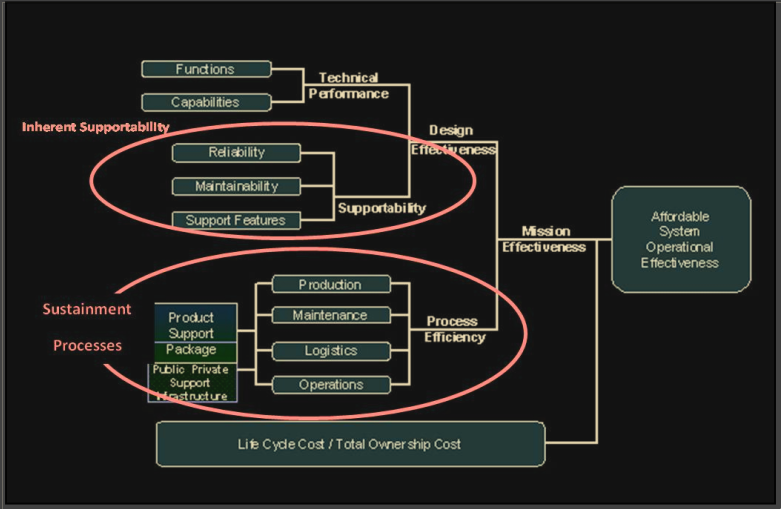
\includegraphics[width=0.8\textwidth]{fig1.png}
\end{center}
\end{frame}

%------------------------------------------------

\begin{frame}{Планирование поддержки}
\begin{itemize}
    \item Влияние на дизайн системы
    \item Планирование процессов поддержки
\end{itemize}

\end{frame}

%------------------------------------------------

\begin{frame}{Факторы поддерживаемости}
\begin{itemize}
    \item Надежность
    \item Ремонтопригодность
    \item Безопасность
    \item Персонал
\end{itemize}

\vspace{0.5cm}

+ среда и диагностика

\end{frame}

%------------------------------------------------

\begin{frame}{Архитектурные решения}
\begin{itemize}
    \item Модульность
    \item Масштабируемость
    \item Открытость
\end{itemize}

\vspace{0.5cm}

Компромисс:
\begin{itemize}
    \item Стоимость vs гибкость
\end{itemize}

\end{frame}

%------------------------------------------------

\begin{frame}{Надежность}
\begin{itemize}
    \item Влияет на доступность
    \item Снижает логистическую нагрузку
\end{itemize}

\vspace{0.5cm}

Цель:
\begin{itemize}
    \item Минимизация отказов
\end{itemize}

\end{frame}

%------------------------------------------------

\begin{frame}{Ремонтопригодность}
\begin{itemize}
    \item Снижение затрат
    \item Быстрое восстановление
\end{itemize}

\vspace{0.5cm}

Ключ:
\begin{itemize}
    \item Встроена в дизайн
\end{itemize}

\end{frame}

%------------------------------------------------

\begin{frame}{Принципы ремонта}
\begin{itemize}
    \item Модульность (replace)
    \item Совместимость
    \item Простота доступа
\end{itemize}

\end{frame}

%------------------------------------------------

\begin{frame}{Дополнительные аспекты}
\begin{itemize}
    \item Минимизация обслуживания
    \item Встроенное тестирование
    \item Интеграция человека (HSI)
\end{itemize}

\end{frame}

%------------------------------------------------

\begin{frame}{Компоненты логистики}
\begin{itemize}
    \item Управление рисками
    \item Инжиниринг поддержки
    \item Снабжение
    \item Документация
\end{itemize}

\end{frame}

%------------------------------------------------

\begin{frame}{Поддержка системы}
\begin{itemize}
    \item Персонал
    \item Обучение
    \item Инфраструктура
    \item IT-ресурсы
\end{itemize}

\end{frame}

%------------------------------------------------

\begin{frame}{Реализация поддержки}
\begin{itemize}
    \item Выполнение планов
    \item Обеспечение требований
    \item Оптимизация затрат
\end{itemize}

\end{frame}

%------------------------------------------------

\begin{frame}{IPS элементы}
\begin{itemize}
    \item Управление поддержкой
    \item Обслуживание
    \item Снабжение
    \item Обучение
\end{itemize}

\vspace{0.5cm}

Всего: 12 элементов

\end{frame}

%------------------------------------------------

\begin{frame}{Процесс SE}
\begin{itemize}
    \item Требования
    \item Архитектура
    \item Верификация
\end{itemize}

\vspace{0.5cm}

+ управление и инфраструктура

\end{frame}

%------------------------------------------------

\begin{frame}{Деятельность SE}
\begin{itemize}
    \item Сбор данных
    \item Анализ проблем
    \item Корректирующие действия
\end{itemize}

\end{frame}

%------------------------------------------------

\begin{frame}{Улучшение системы}
\begin{itemize}
    \item Тестирование решений
    \item Оценка рисков
    \item Внедрение
\end{itemize}

\end{frame}

%------------------------------------------------

\begin{frame}{Иллюстрация поддержки}
\begin{center}
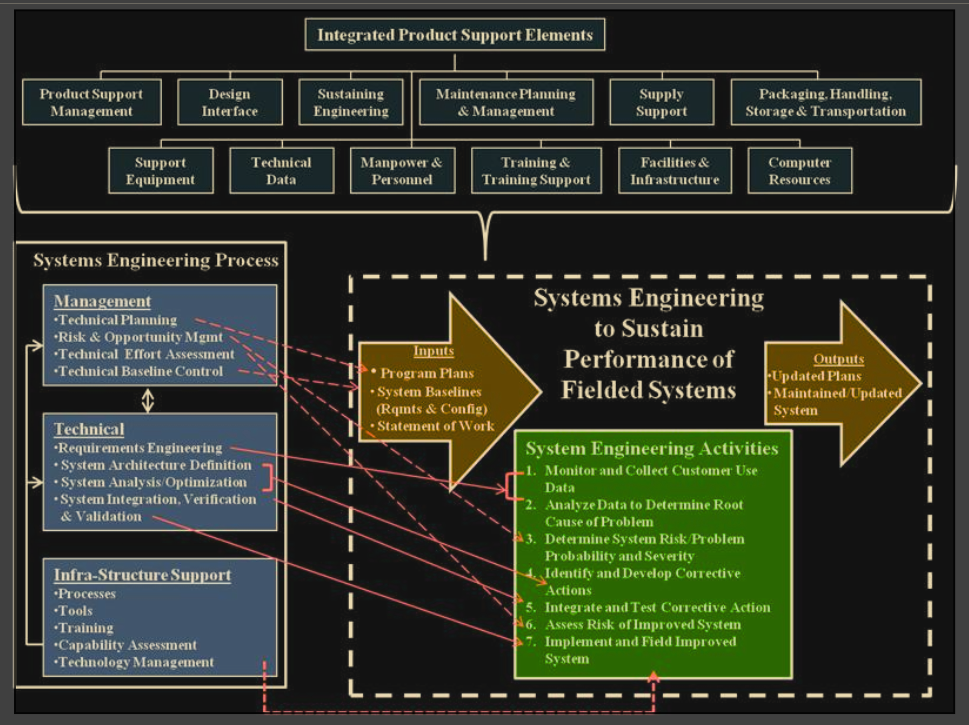
\includegraphics[width=0.8\textwidth]{fig2.png}
\end{center}
\end{frame}

%------------------------------------------------

\begin{frame}{Изменения системы}
\begin{itemize}
    \item Мелкие (процедуры)
    \item Крупные (перепроектирование)
\end{itemize}

\vspace{0.5cm}

Всегда:
\begin{itemize}
    \item Учет IPS элементов
\end{itemize}

\end{frame}

%------------------------------------------------

\begin{frame}{Эволюционные системы}
\begin{itemize}
    \item Поэтапное развитие
    \item Расширение функций
\end{itemize}

\vspace{0.5cm}

Подход:
\begin{itemize}
    \item System of Systems
\end{itemize}

\end{frame}

%------------------------------------------------

\begin{frame}{Вывод}
\begin{itemize}
    \item Логистика влияет на дизайн
    \item Поддержка = часть системы
    \item Ключ — интеграция процессов
\end{itemize}

\end{frame}

\end{document}
